% Created 2022-05-24 mar 18:57
% Intended LaTeX compiler: pdflatex
\documentclass[presentation]{beamer}
\usepackage[utf8]{inputenc}
\usepackage[T1]{fontenc}
\usepackage{graphicx}
\usepackage{grffile}
\usepackage{longtable}
\usepackage{wrapfig}
\usepackage{rotating}
\usepackage[normalem]{ulem}
\usepackage{amsmath}
\usepackage{textcomp}
\usepackage{amssymb}
\usepackage{capt-of}
\usepackage{hyperref}
\logo{\includegraphics[height=0.5cm]{./assets/lOGO-HORIZONTAL-KONRAD-COLOR.jpg}}
\usepackage[spanish]{babel}
\usetheme[height=20pt]{Rochester}
\author{Jonatan Ahumada}
\date{\today}
\title{Modelo de literariedad basado en la lingüistica de Roman Jakobson}
\subtitle{Fundación Universitaria Konrad Lorenz}
\hypersetup{
 pdfauthor={Jonatan Ahumada},
 pdftitle={Modelo de literariedad basado en la lingüistica de Roman Jakobson},
 pdfkeywords={},
 pdfsubject={},
 pdfcreator={Emacs 27.2 (Org mode 9.4.4)}, 
 pdflang={Spanish}}
\begin{document}

\maketitle
\begin{frame}{Outline}
\tableofcontents
\end{frame}



\section{Introducción}
\label{sec:orgc23f93c}

\begin{frame}[label={sec:orge57e06b}]{¿Qué es \emph{literariedad}?}
Es una presunta \emph{característica} que distingue un texto literario de
otro no literario.

Por ejemplo:

\begin{itemize}
\item Manual de un carro vs. un poema de Jose Asunción Silva (fácil)
\item Artículo periodístico  vs. cuento corto  (normal)
\item \emph{50 sombras de Gray} vs. \emph{Ulysses} (difícil)
\end{itemize}
\end{frame}


\begin{frame}[label={sec:org34f53a8}]{Antecedentes: Los clásicos}
En los estudios clásicos, se encuentran teorías acerca de qué constituye
un texto 'poético' o una buena 'narración'.

\begin{itemize}
\item Fedro, Platón
\item Póetica, Aristóteles
\item Carta a los pisones, Horacio
\end{itemize}

Sin embargo, el enfoque que toman estos autores no es \alert{metódico} o \alert{sistemático}
\end{frame}

\begin{frame}[label={sec:orga1c2670}]{Antecedentes: la linguística estructural}
En el siglo 20, Ferdinand de Saussure fundó la linguística general
(también llamada estructural). Se considera al fenómeno del
lenguaje como una estructura compuesta de varios componentes
interdependientes, pero identificables.
\end{frame}


\begin{frame}[label={sec:org7c362ad}]{Antecedentes: Roman Jakobson}
\begin{columns}
\begin{column}{0.48\columnwidth}
Roman Jakobson fue un lingüista ruso americano. Se considera una
figura clave tanto en movimiento del \emph{formalismo ruso}, así como
en el \emph{estructuralista}.  La lingüística de Jakobson se basa en
los postulados de la lingüistica de Saussure, \alert{pero} propuso una
crítica a las ideas de Saussure.
\end{column}


\begin{column}{0.48\columnwidth}
\begin{block}{Cita}
\begin{quote}
The fundamental role which these two operations play in language
was clearly realized by Ferdinand de Saussure. Yet of the two
varieties of combination-concurrence and concatenation-it was only
the latter, the temporal sequence, which was recognized by the
Geneva linguist. 
\cite[p. 99]{jakobson1956two}
\end{quote}
\end{block}
\end{column}
\end{columns}
\end{frame}




\begin{frame}[label={sec:org4a753b9}]{La pregunta}
\begin{block}{}
   ¿Cómo medir
   computarizadamente la \emph{literariedad} de un texto según el marco de la
   lingüística de Jakobson?
\end{block}
\end{frame}


\section{Objetivos}
\label{sec:org296dc80}
\begin{frame}[label={sec:org87b3a6d}]{General}
   \begin{block}{General}

Diseñar e implementar un modelo que, dado un corpus de texto, produzca
   indicadores para el concepto de \emph{literariedad} que plantea Roman Jakobson.
     \end{block}
\end{frame}

\begin{frame}[label={sec:org5f39379}]{Específicos}
\begin{enumerate}
\item Construir el corpus necesario para representar el \emph{eje sincrónico}.
\item Diseñar e implementar el algoritmo para calcular la \emph{metáfora} sobre un corpus.
\item Diseñar e implementar algoritmo para calcular la \emph{metonimia} sobre un corpus.
\item Seleccionar y unir los textos que serán procesados (corpus objetivo) por el algoritmo.
\item Correr el algoritmo sobre los corpus objetivo.
\item Evaluar el algoritmo de manera cuantitativa y cualitativa.
\end{enumerate}
\end{frame}

\begin{frame}[label={sec:org9934527}]{Alcance}
\begin{enumerate}
\item Modelos \alert{naive}

\item Corpus de acceso libre (Brown Corpus)

\item Herramientas 'básicas' de NLP. (no Machine Learning)
\end{enumerate}
\end{frame}


\section{Marco teórico y referencial}
\label{sec:org571db8d}

\begin{frame}[label={sec:org703b308}]{Introducción a metáfora y metonimia}
\begin{columns}
\begin{column}{0.48\columnwidth}
   \begin{figure}
  \caption{\emph{Cisnes reflejando elefantes} de Salvador Dalí}
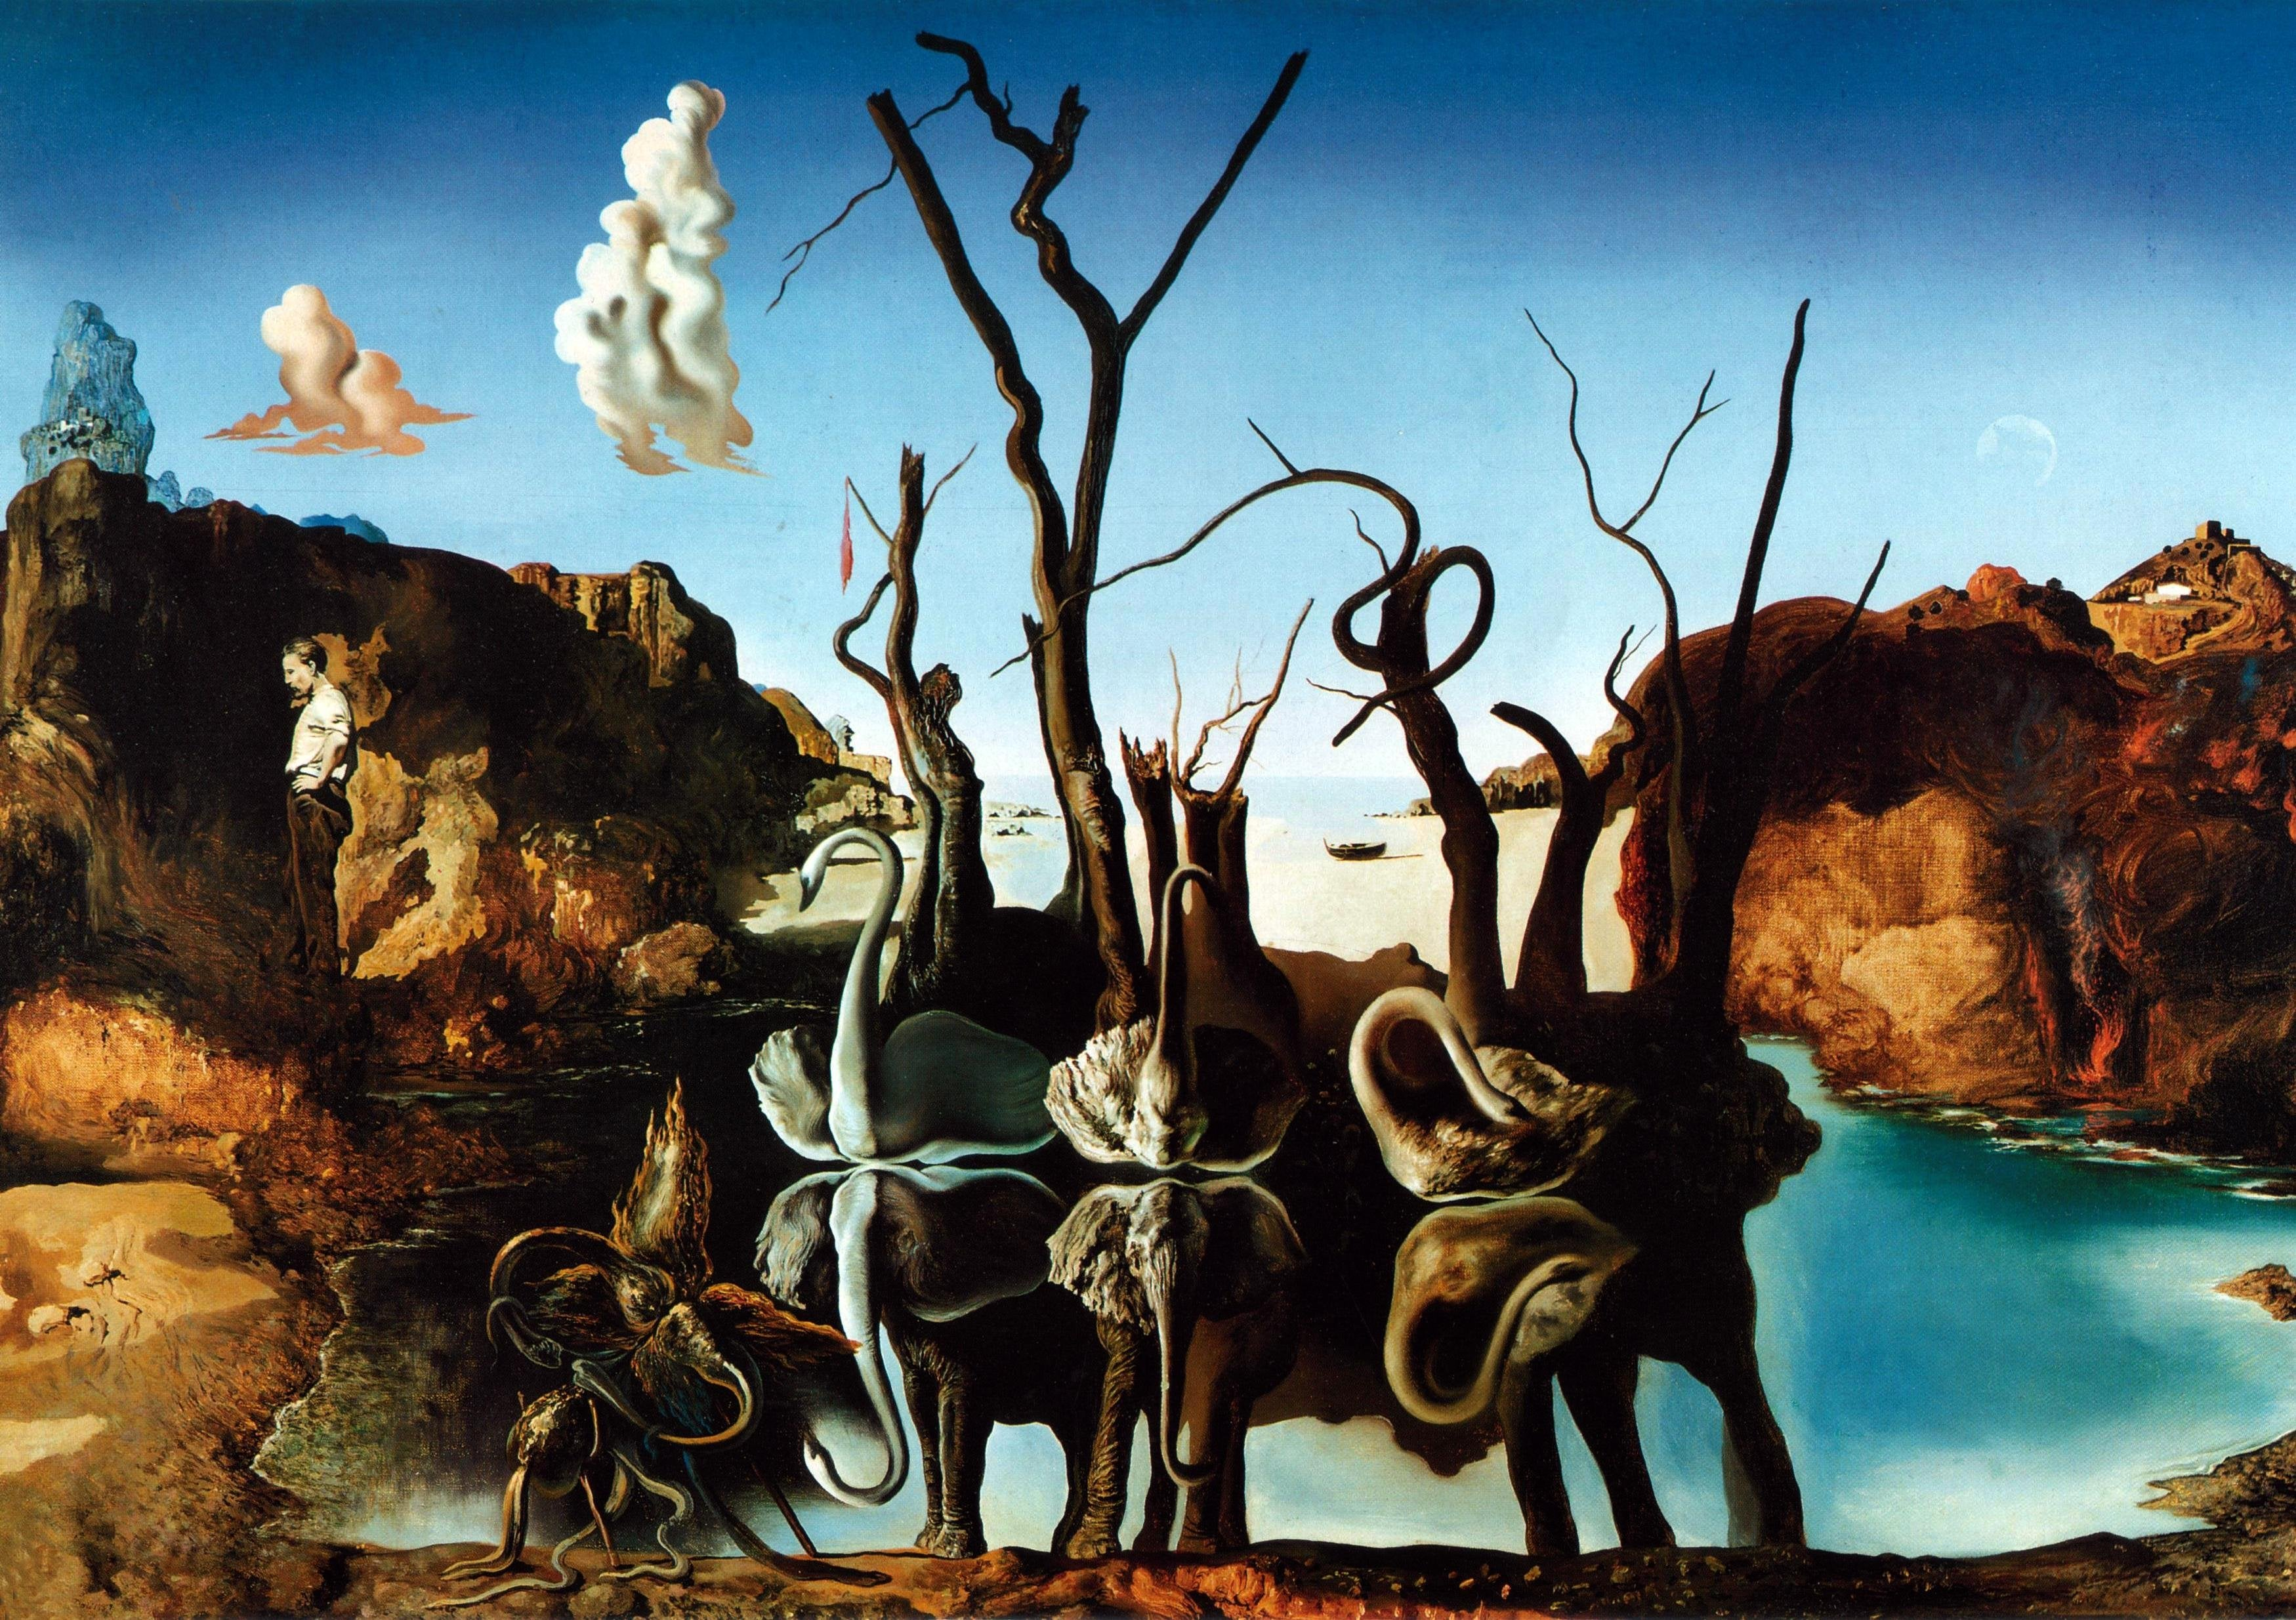
\includegraphics[width=\textwidth]{./assets/arte_dali.jpg}

   \end{figure}
\end{column}

\begin{column}{0.48\columnwidth}
\begin{figure}
    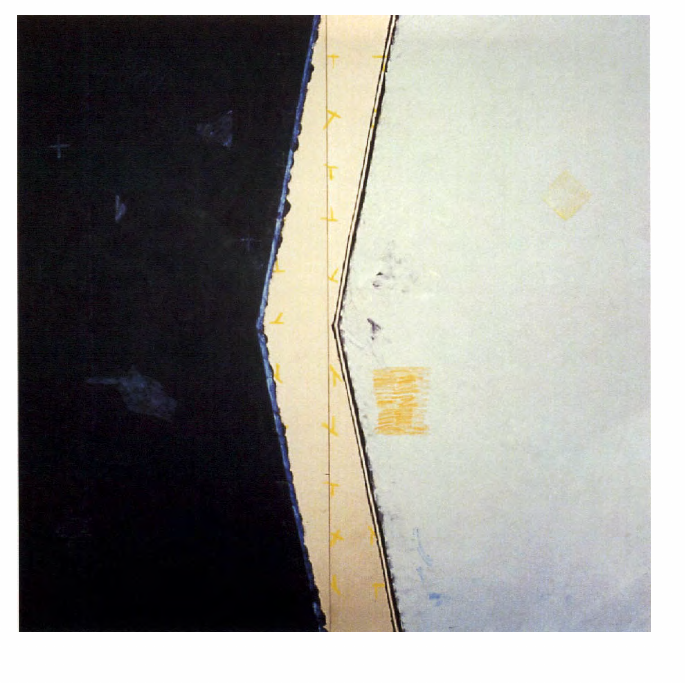
\includegraphics[width=\textwidth]{./assets/arte_green.png}
\caption{\emph{9 grados} de Denise Green}
 \end{figure}
\end{column}
\end{columns}
\end{frame}

\begin{frame}[label={sec:orgdaa1b50}]{Metáfora y metonimia}
\begin{columns}
\begin{column}{0.48\columnwidth}
\begin{figure}
    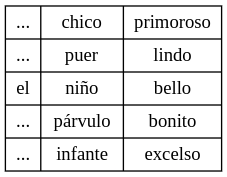
\includegraphics[width=0.6\textwidth]{./assets/ejemplo_metafora.png}
\caption{Ejemplo de metáfora}
 \end{figure}

 \begin{figure}
    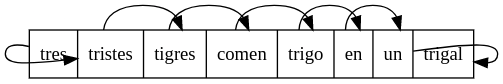
\includegraphics[width=\textwidth]{./assets/ejemplo_metonimia.png}
\caption{Ejemplo de metonimia}
 \end{figure}
\end{column}


\begin{column}{0.48\columnwidth}
\tiny

      \begin{block}{Selección/Metáfora}
A selection between alternatives implies the possibility
of substituting one for the other, equivalent in one respect and differ­
ent in another. Actually, selection and substitution are two faces of the
same operation. \cite[p.98]{jakobson1956two}


   \end{block}

   \begin{block}{Combinación/Metonimia}
Any linguistic sign involves two modes of arrangement: Any sign is made up of constituent signs and/or
occurs only in combination with other signs. This means that any lin­
guistic unit at one and the same time serves as a context for simpler
units and/or finds its own context in a more complex linguistic unit.
\cite[p.99]{jakobson1956two}
   \end{block}



\normalsize
\end{column}
\end{columns}
\end{frame}

\section{Diseño Metodológico}
\label{sec:orgcbf3a20}

\begin{frame}[label={sec:org00d07a2}]{CRISP-DM}
\begin{figure}
\caption{Pasos de CRISP-DM}
 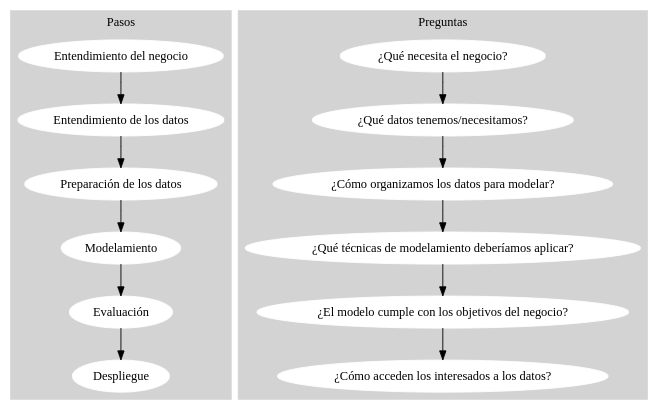
\includegraphics[width=0.8\textwidth]{./assets/metodologia.png}

 \end{figure}
\end{frame}

\section{Entendimiento del negocio}
\label{sec:org6469e9d}
\begin{frame}[label={sec:org698a3cd}]{Entendimiento del negocio}
Cada algoritmo recibe un mensaje  \(m\) de entrada con:
\begin{block}{Entrada}
\begin{itemize}
\item cadena de cualquier longitud
\item sin POS
\item sin set de entrenamiento
\end{itemize}
\end{block}
produce:

\begin{block}{Salida}
\begin{itemize}
\item  Un valor continuo para dicho mensaje (no es categórico)
\item  Entre más alto el valor, más fuerte es esa característica (metáfora y/o metonímia)
\end{itemize}
\end{block}
\end{frame}

\begin{frame}[label={sec:org7f5ae6c}]{Casos de uso}
  \begin{figure}
   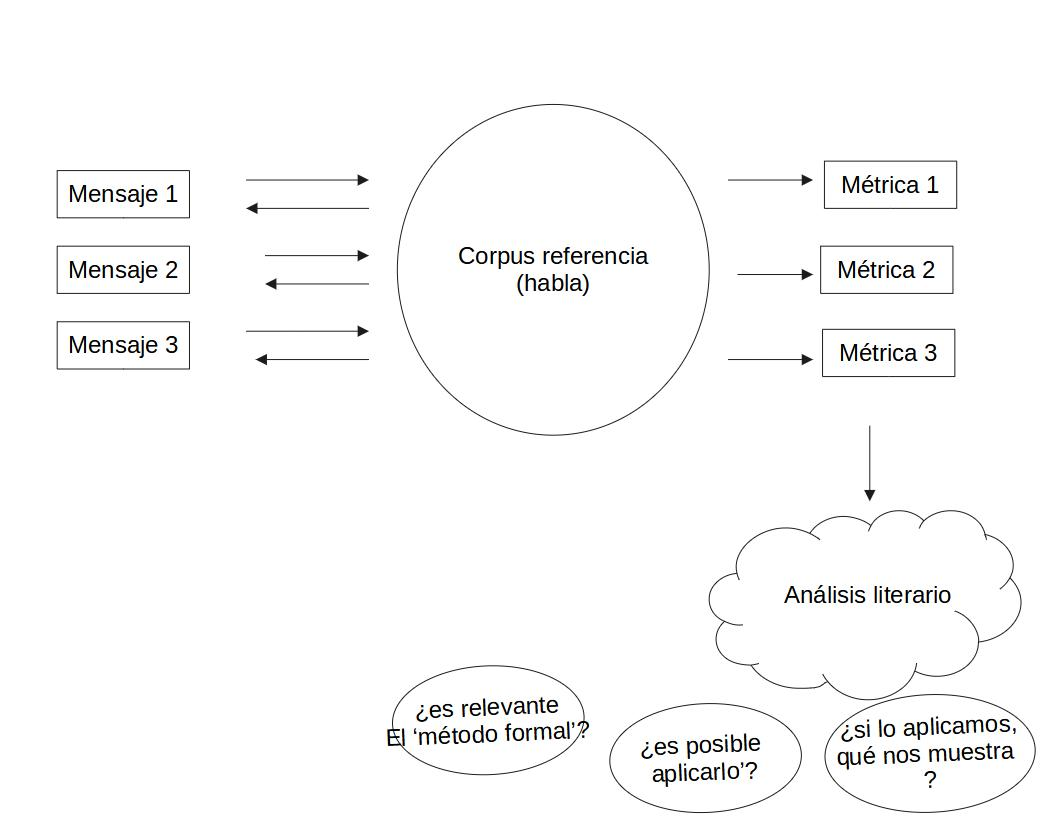
\includegraphics[width=\textwidth]{./assets/posibles_usos.jpg}

\end{figure}
\end{frame}

\begin{frame}[label={sec:org4eb2328}]{Usuarios}
  \begin{figure}
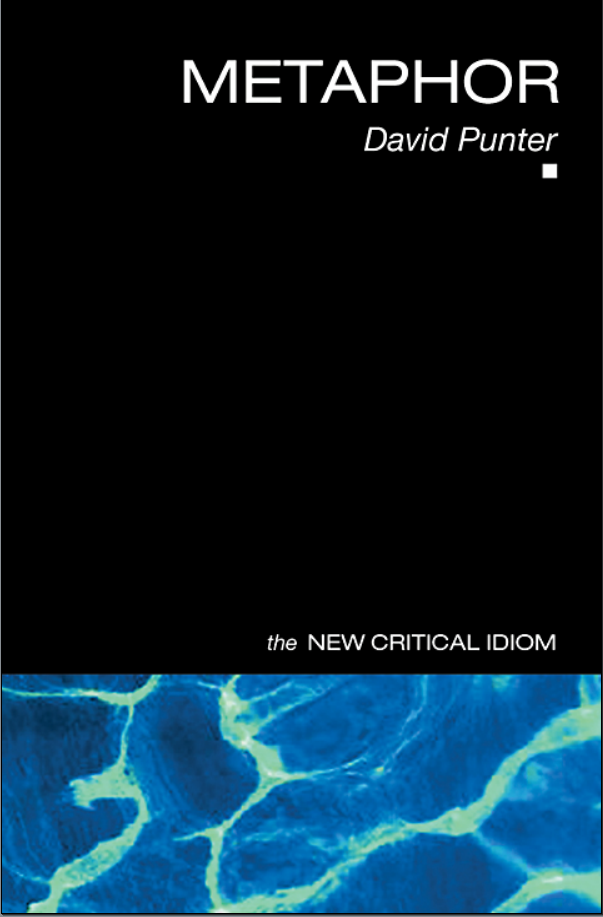
\includegraphics[width=0.24\textwidth]{./assets/negocio_metafora1.png}
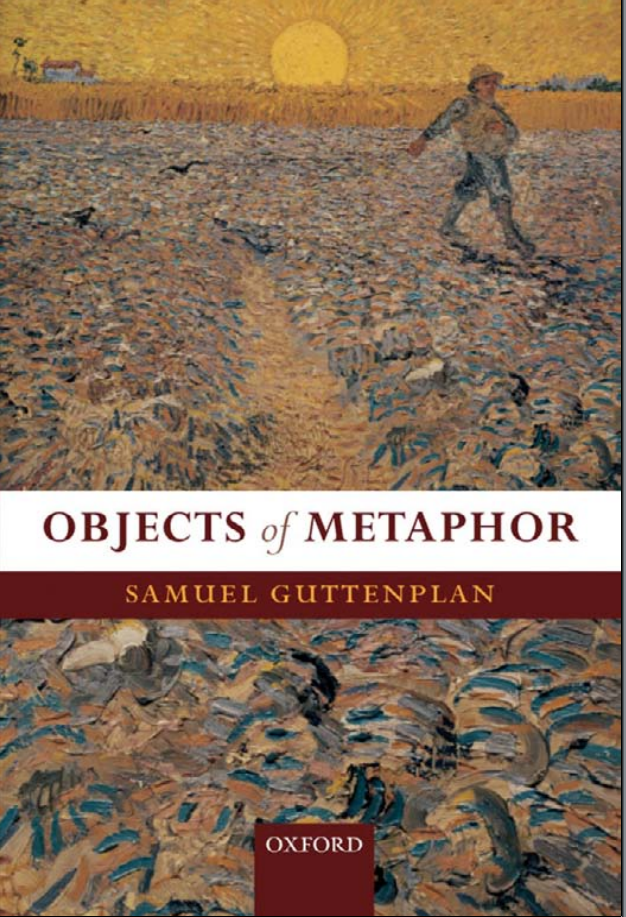
\includegraphics[width=0.24\textwidth]{./assets/negocio_metafora2.png}
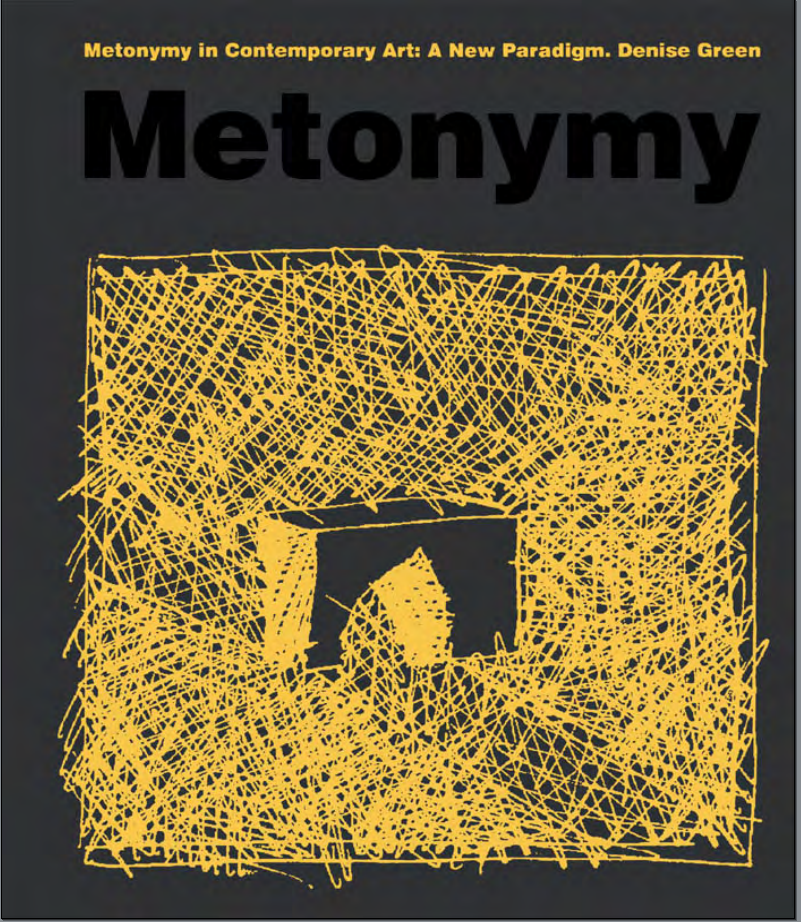
\includegraphics[width=0.24\textwidth]{./assets/negocio_metonimia1.png}
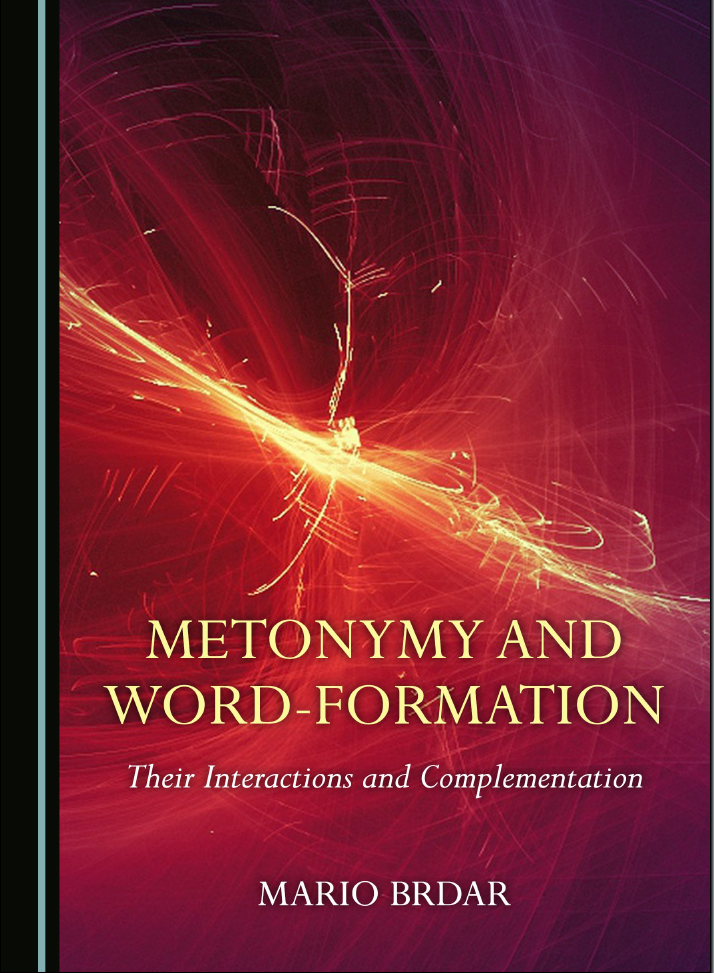
\includegraphics[width=0.24\textwidth]{./assets/negocio_metonimia2.png}
  \end{figure}
\end{frame}

\section{Entendimiento de los datos}
\label{sec:org4072b42}
\begin{frame}[label={sec:orgdb32106}]{Entendimiento de los datos}
\begin{columns}
\begin{column}{0.48\columnwidth}
Son esencialmente 3 componentes:

\begin{block}{Corpus de referencia}
Modela el estado actual de la \emph{lengua}.
Eje de sicnronía en Saussure.
\end{block}

\begin{block}{Red semántica}
 Modela el lenguaje: la capacidad de asociar ideas con símbolos.
\end{block}

\begin{block}{Corpus objetivo}
 Modela el \emph{habla}. El mensaje que será sometido a análisis.
\end{block}
\end{column}



\begin{column}{0.48\columnwidth}
\begin{figure}
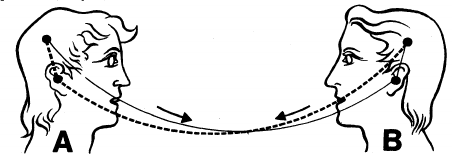
\includegraphics[width=\textwidth]{./assets/sistema-comunicacion.png}
\caption{El circuito linguístico. Tomado de \cite{alonso1945curso}}
\end{figure}

   \begin{figure}

   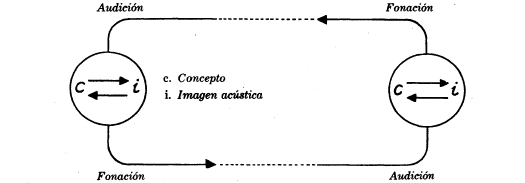
\includegraphics[width=\textwidth]{./assets/sistema-comunicacion2.png}
\caption{El circuito linguístico (visión alterna). Tomado de \cite{alonso1945curso}}
   \end{figure}
\end{column}
\end{columns}
\end{frame}

\begin{frame}[label={sec:org3db16b7}]{Resumen}
\begin{figure}
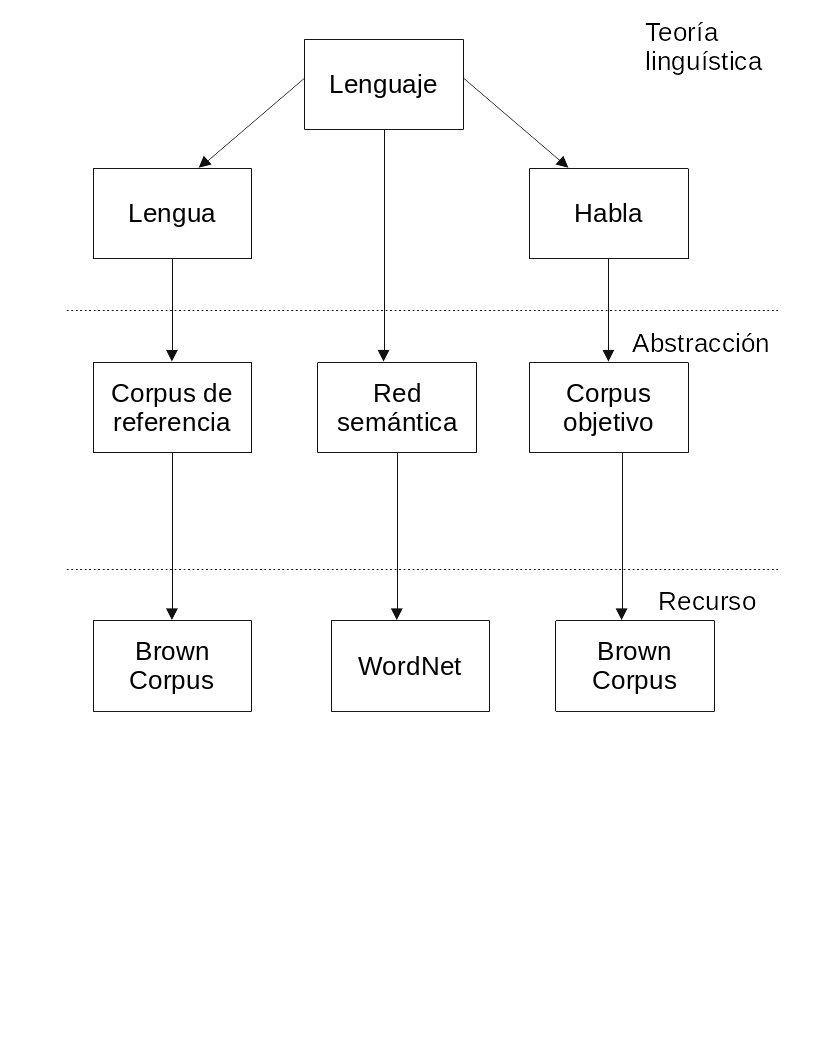
\includegraphics[height=\textheight]{./assets/entendimiento_de_los_datos.png}

\end{figure}
\end{frame}

\begin{frame}[label={sec:orgace1785}]{Corpus Brown}
Se seleccionó porque:
\small
\begin{itemize}
\item todas las muestras del corpus pertenecen al año 1961,
\item todas las muestras del corpus se imprimieron en Estados Unidos durante ese año,
\item todos los autores son hablantes nativos de inglés,
\item la categorización de las muestras fue hecha por un comité de expertos de la universidad de Brown,
\item la intención declarada del corpus es la de ser una muestra representativa del inglés de aquel año,
\item tiene una lista amplia de categorías que podrían ser útiles para observar diferencias entre las categorías,
\item los resultados obtenidos del modelo podrían ser replicados porque el corpus es ampliamente conocido.
\item el número de textos por categoría guarda la relación entre los textos publicados de esa categoría durante ese año y
\item los resultados obtenidos del modelo podrían ser replicados porque el corpus es ampliamente conocido.
\end{itemize}
\normalsize
\end{frame}

\begin{frame}[label={sec:orgd985e9e}]{Wordnet}
\begin{columns}
\begin{column}{0.48\columnwidth}
    \begin{block}{Definición}
Es una base de datos de \emph{relaciones conceptuales} entre palabras.
\end{block}


\begin{block}{Cita}
Wordnet's design resembles that of a thesaurus in that its building block is a synset consisting of all the
words that express a given concepts (...) The synsets are linked by means of a number of relations,
including, hyponymy, meronymy and entailment.     \cite[p.8]{fellbaum_1998}
\end{block}
\end{column}


\begin{column}{0.48\columnwidth}
\begin{figure}
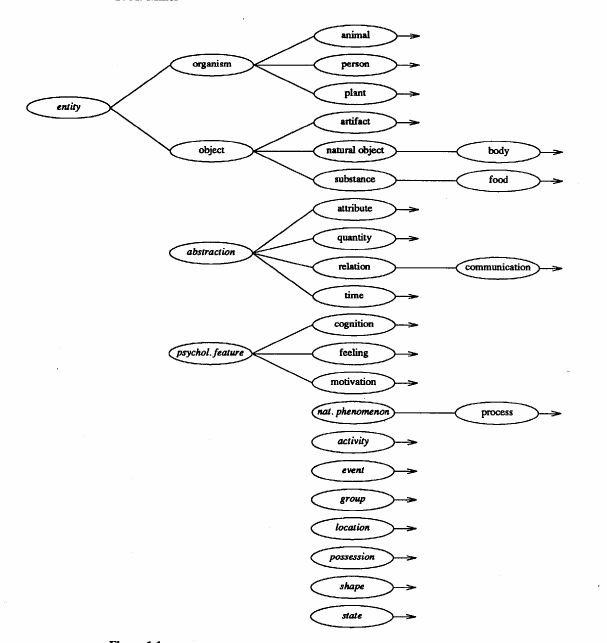
\includegraphics[width=0.7\textwidth]{./assets/wordnet-relaciones.png}
\caption{Ejemplo de relaciones entre conceptos en Wordnet. Tomado de \cite[p.30]{fellbaum_1998}}
\end{figure}
\end{column}
\end{columns}
\end{frame}
\section{Preparación de los datos}
\label{sec:org9c90d98}
\begin{frame}[label={sec:org0b38195}]{Preparación de los datos}
\begin{figure}
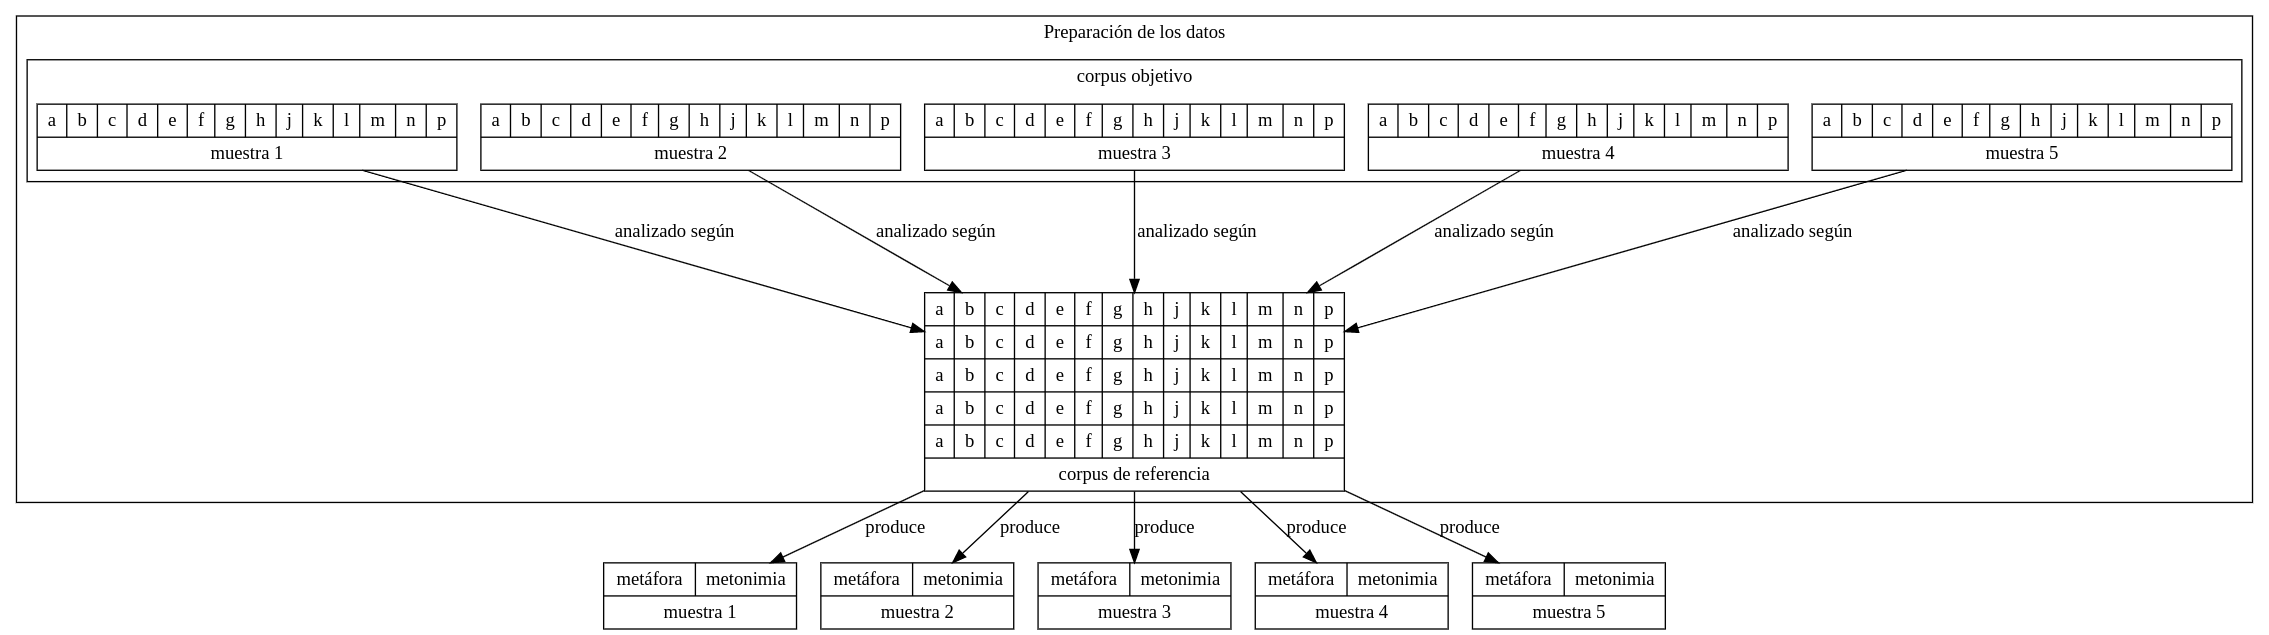
\includegraphics[width=\textwidth]{./assets/preparacion_visualizacion.png}
\end{figure}

\begin{block}{¿En qué consistió la preparación?}
\begin{itemize}
\item Conformar el corpus de referencia
\item Conformar los corpus objetivo
\item Controlar la mayor cantidad de variables
\end{itemize}
\end{block}
\end{frame}
\begin{frame}[label={sec:org28ff059}]{Resumen}
     \begin{table}[!ht]
    \centering

    \begin{tabular}{|c|c|}
    \hline
      Atributo & Cantidad \\ \hline
      Textos en corpus de referencia & 60 \\ \hline
      Categorías en corpus de referencia  & 13 \\ \hline
     Textos en corpus objetivo & 70 \\ \hline
     Textos en muestra de corpus objetivo & 14 \\ \hline
     Muestras de corpus objetivo & 5 \\ \hline
     Categorías por muestra & 14  \\ \hline
     Total de textos usados & 130  \\ \hline
    \end{tabular}
\caption{Resumen de datos utilizados}
\label{tab:resumen_preparacion}
\end{table}
\end{frame}

\section{Modelamiento}
\label{sec:orgd6d398b}
\begin{frame}[label={sec:orga33e5c4}]{Modelamiento}
\begin{columns}
\begin{column}{0.48\columnwidth}
\tiny
    \begin{block}{Metáfora}
\begin{equation}
\label{eq:mensaje}
mensaje = \{ w_1, w_2, w_3, \dots , w_j \}
\end{equation}

\begin{equation}
\label{eq:vector_semantico}
vector\ semantico(w) = \{s_1, s_2, s_3, \dots, s_j \} 
\end{equation}

\begin{equation}
\label{eq:vector_uso}
vector\ uso(w) = \{freq_{ref}(s_1),freq_{ref}(s_2),freq_{ref}(s_3), \dots, freq_{ref}(s_j) \} 
\end{equation}

\begin{equation}
\label{eq:promedio}
\mu = \frac{\Sigma_i^jfreq_{referencia}(s_i)}{j}
\end{equation}


\begin{equation}
\label{eq:uso}
uso(w) = \frac{freq_{objetivo}(w)}{\mu}
\end{equation}


\begin{equation}
\label{eq:indice_metafórico}
indice\ metaforico(mensaje) =  \Sigma_i^j uso(w_i)
\end{equation}

\end{block}
\normalsize
\end{column}
\begin{column}{0.48\columnwidth}
     \begin{figure}

\includegraphics[width=\textwidth]{./assets/codigo_vector_semantico.png}
\caption{Ejemplo de implementación}
\end{figure}

   \begin{figure}

   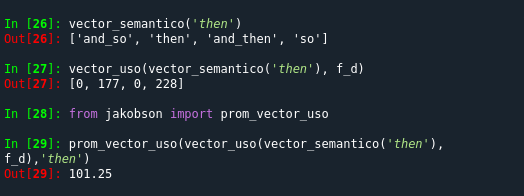
\includegraphics[width=\textwidth]{./assets/codigo_vector_uso.png}
\caption{Ejemplo de implementación}
   \end{figure}
\end{column}
\end{columns}
\end{frame}


\begin{frame}[label={sec:org61840b4}]{Modelamiento}
\begin{columns}
\begin{column}{0.48\columnwidth}
\tiny
\begin{block}{Metonimia}
\begin{equation}
\label{eq:ngramas}
N = \{n_1, n_2, n_3, \dots , n_j\}
\end{equation}

\begin{equation}
\label{eq:metonimia}
met(n_i) = \frac{letras\ iguales}{ set(letras(n_i1) + letras(n_i2))}
\end{equation}

\begin{equation}\label{eq:indice_metonimia}
indice\ metonimia = \Sigma_i^j met(n_i)
\end{equation}
\end{block}
\normalsize
\end{column}
\begin{column}{0.48\columnwidth}
\begin{figure}
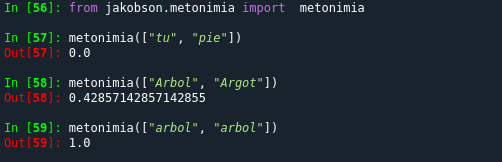
\includegraphics[width=\textwidth]{./assets/codigo_metonimia.png}
\caption{Ejemplo de implementación}
\end{figure}

\begin{figure}

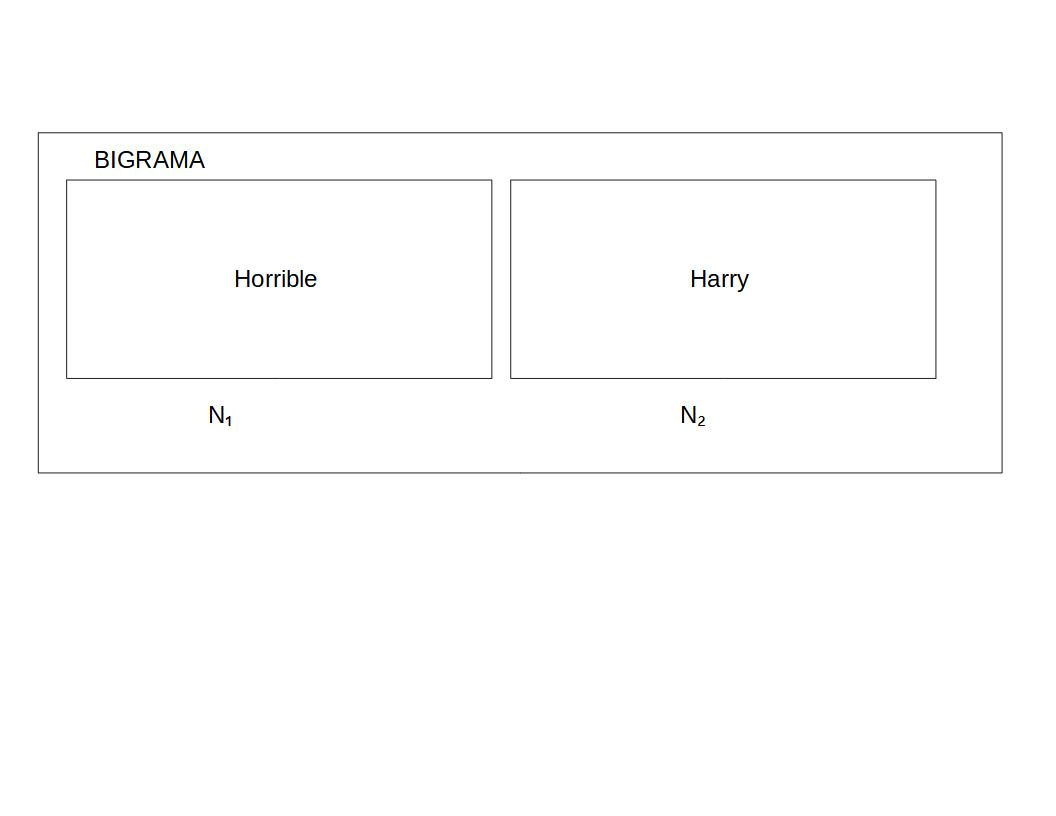
\includegraphics[width=\textwidth]{./assets/metonimia.jpg}
\caption{Concepto de metonimia}
\end{figure}
\end{column}
\end{columns}
\end{frame}

\begin{frame}[label={sec:org0a6cb9a}]{Diseño experimental}
\begin{block}{Criterios cualitativos}
\begin{itemize}
\item H\textsubscript{1}: Se espera que las categorías de ficción tengan un índice metafórico significativamente mayor que los de no-ficción.
\item H\textsubscript{2}: Se espera que las categorias 'Reportage' y 'Editorial' tengan índices metafóricos similares a través de las muestras.
\item H\textsubscript{3}: Se espera que la categoría 'Belles Lettres' tenga un indíce metafórico más alta entre las categorías de no-ficción.
\item H\textsubscript{4}: Se espera que la categoria 'Learned' tenga un indice metonímico bajo en general.
\end{itemize}
\end{block}
\begin{block}{Criterios cuantitativos}
Prueba ANOVA: ¿Los resultados que se obtuvieron son aleatorios?
\end{block}
\end{frame}
\section{Despliegue}
\label{sec:org7904323}
\begin{frame}[label={sec:org1adfccb}]{Resultados por categorías}
\begin{columns}
\begin{column}{0.48\columnwidth}
\begin{figure}[H]
\centering
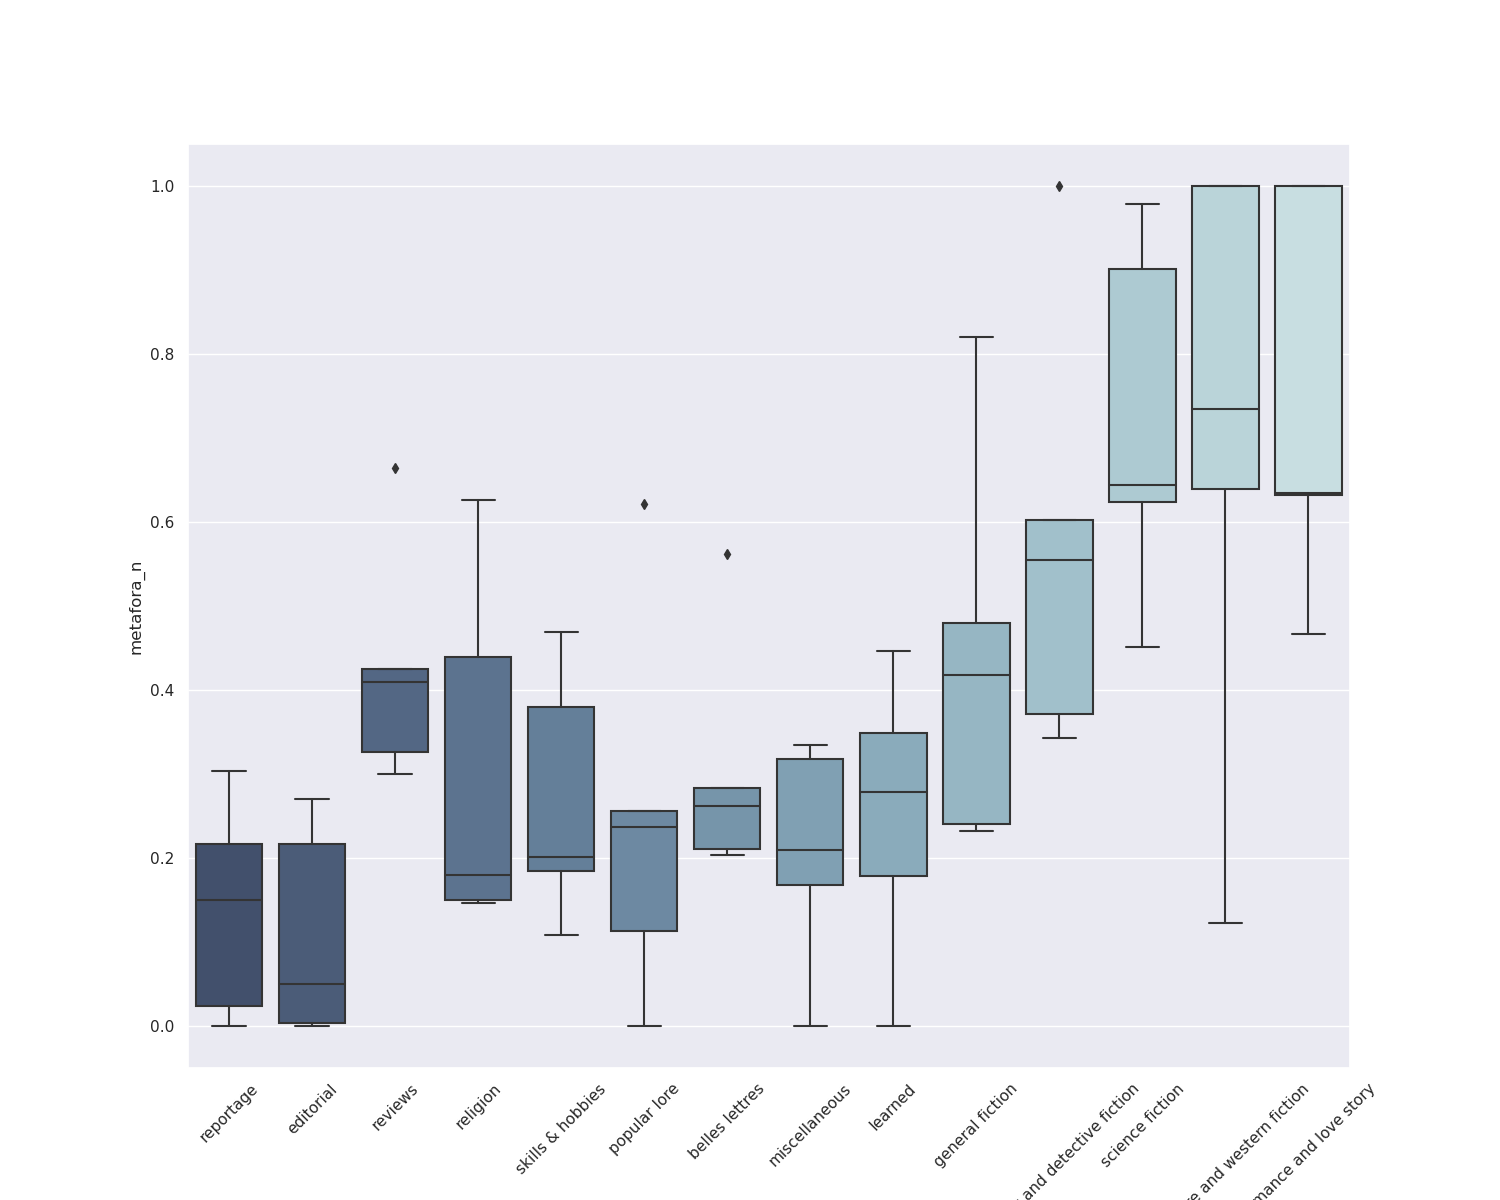
\includegraphics[width=\linewidth]{./resultados/graphs/total/accum_cat_metafora.png}

\caption{Metáfora través de las muestras }
\end{figure}
\end{column}

\begin{column}{0.48\columnwidth}
\begin{figure}[H]
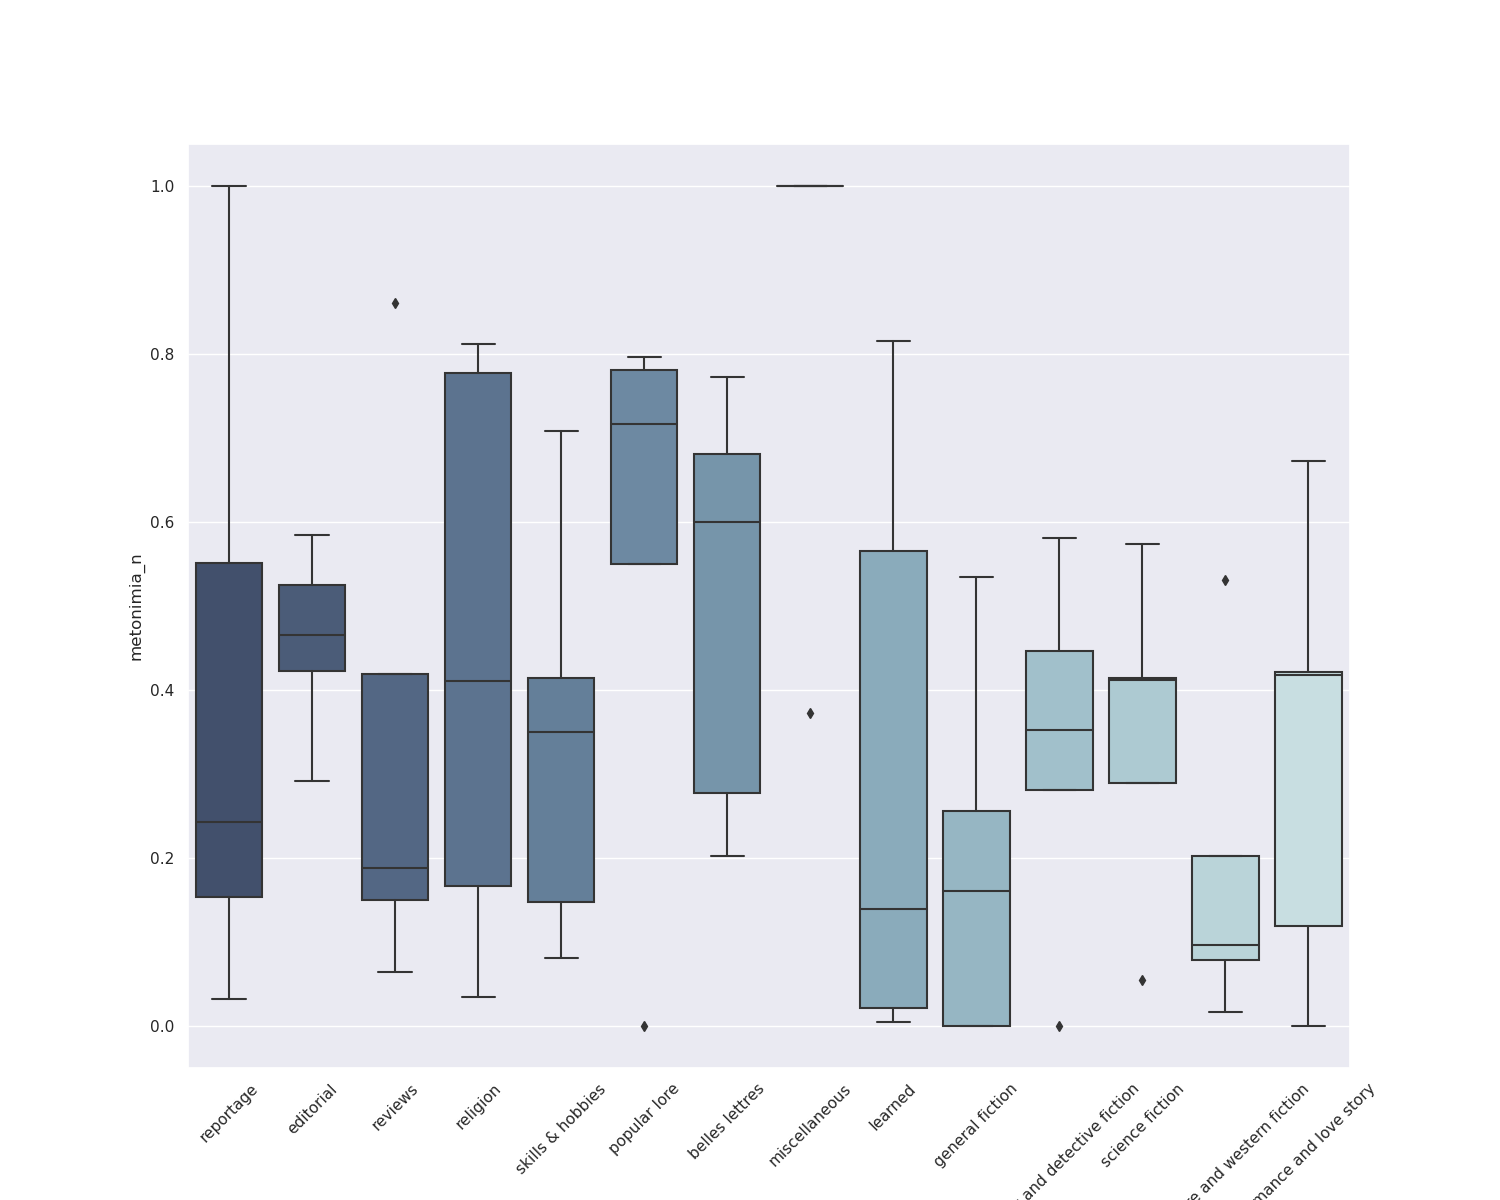
\includegraphics[width=\linewidth]{./resultados/graphs/total/accum_cat_metonimia.png}
\caption{Metonimia través de las muestras }
\centering

\end{figure}
\end{column}
\end{columns}
\end{frame}

\begin{frame}[label={sec:org5d93f95}]{Resultados por metacategorías}
\begin{columns}
\begin{column}{0.48\columnwidth}
\begin{figure}[H]
\centering
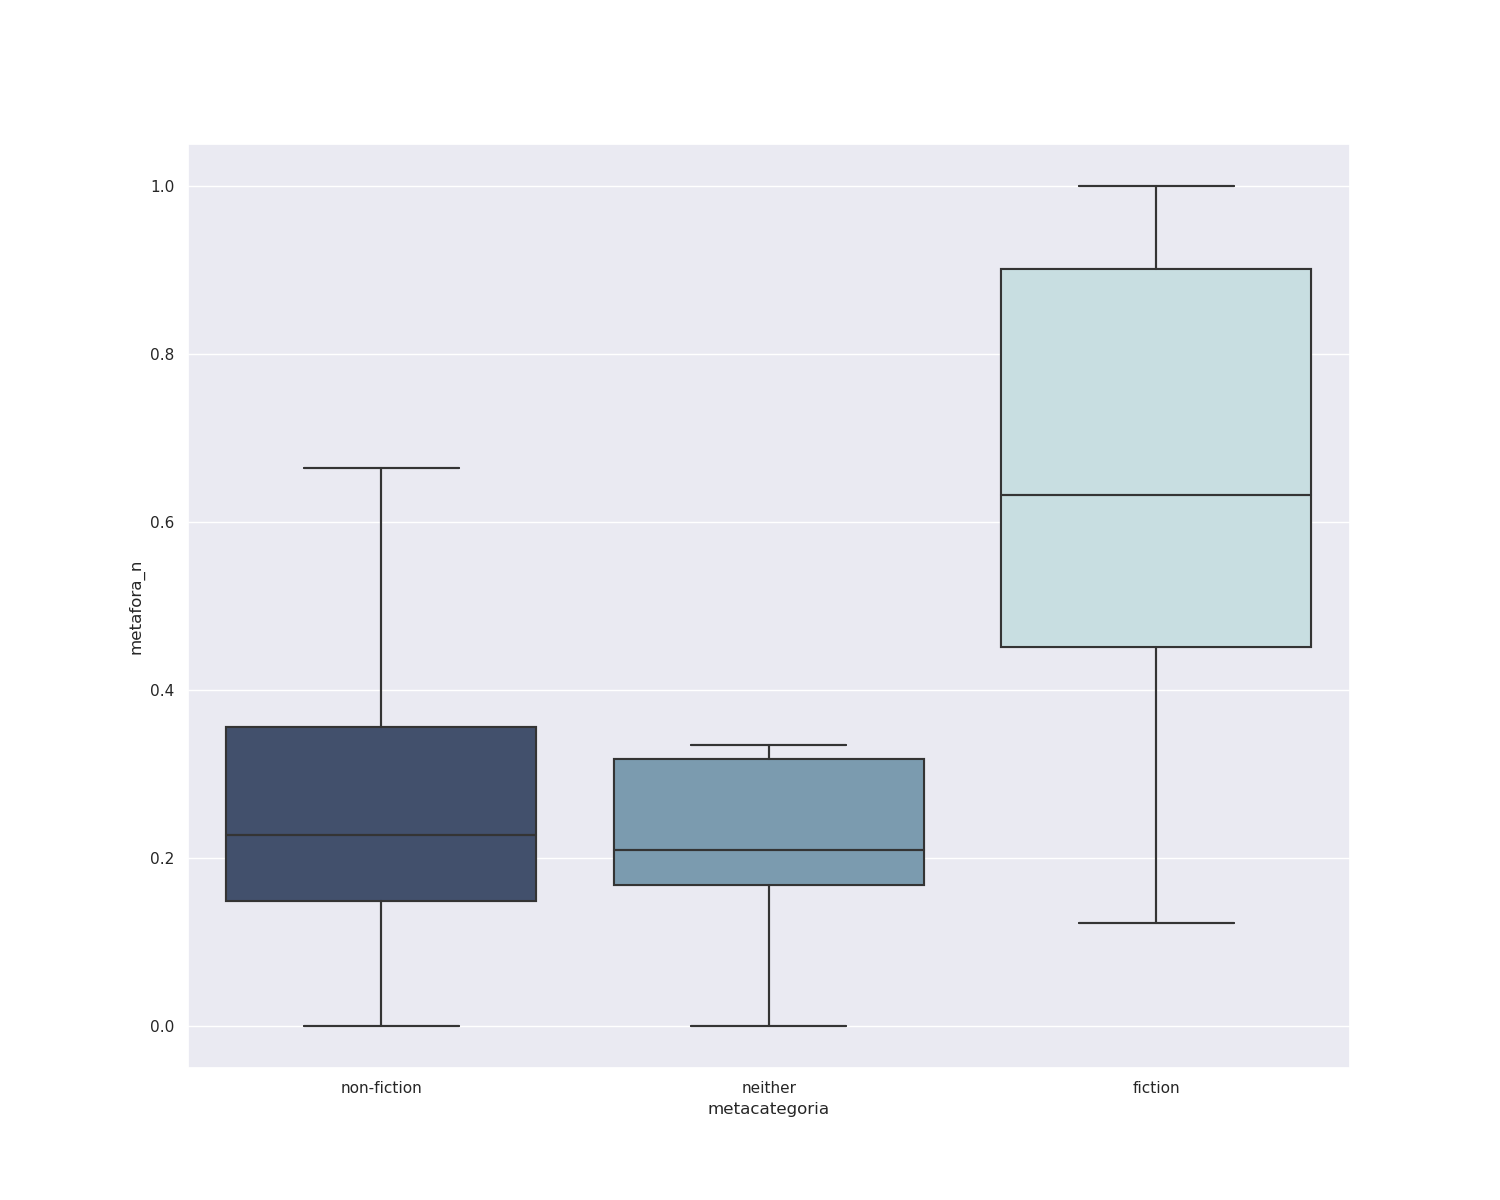
\includegraphics[width=0.9\linewidth]{./resultados/graphs/total/metafora_total.png}
\caption{\label{fig:metafora_total} Índice metafórico por metacategorías a través de muestras }
\end{figure}
\end{column}


\begin{column}{0.48\columnwidth}
\begin{figure}[H]
\centering
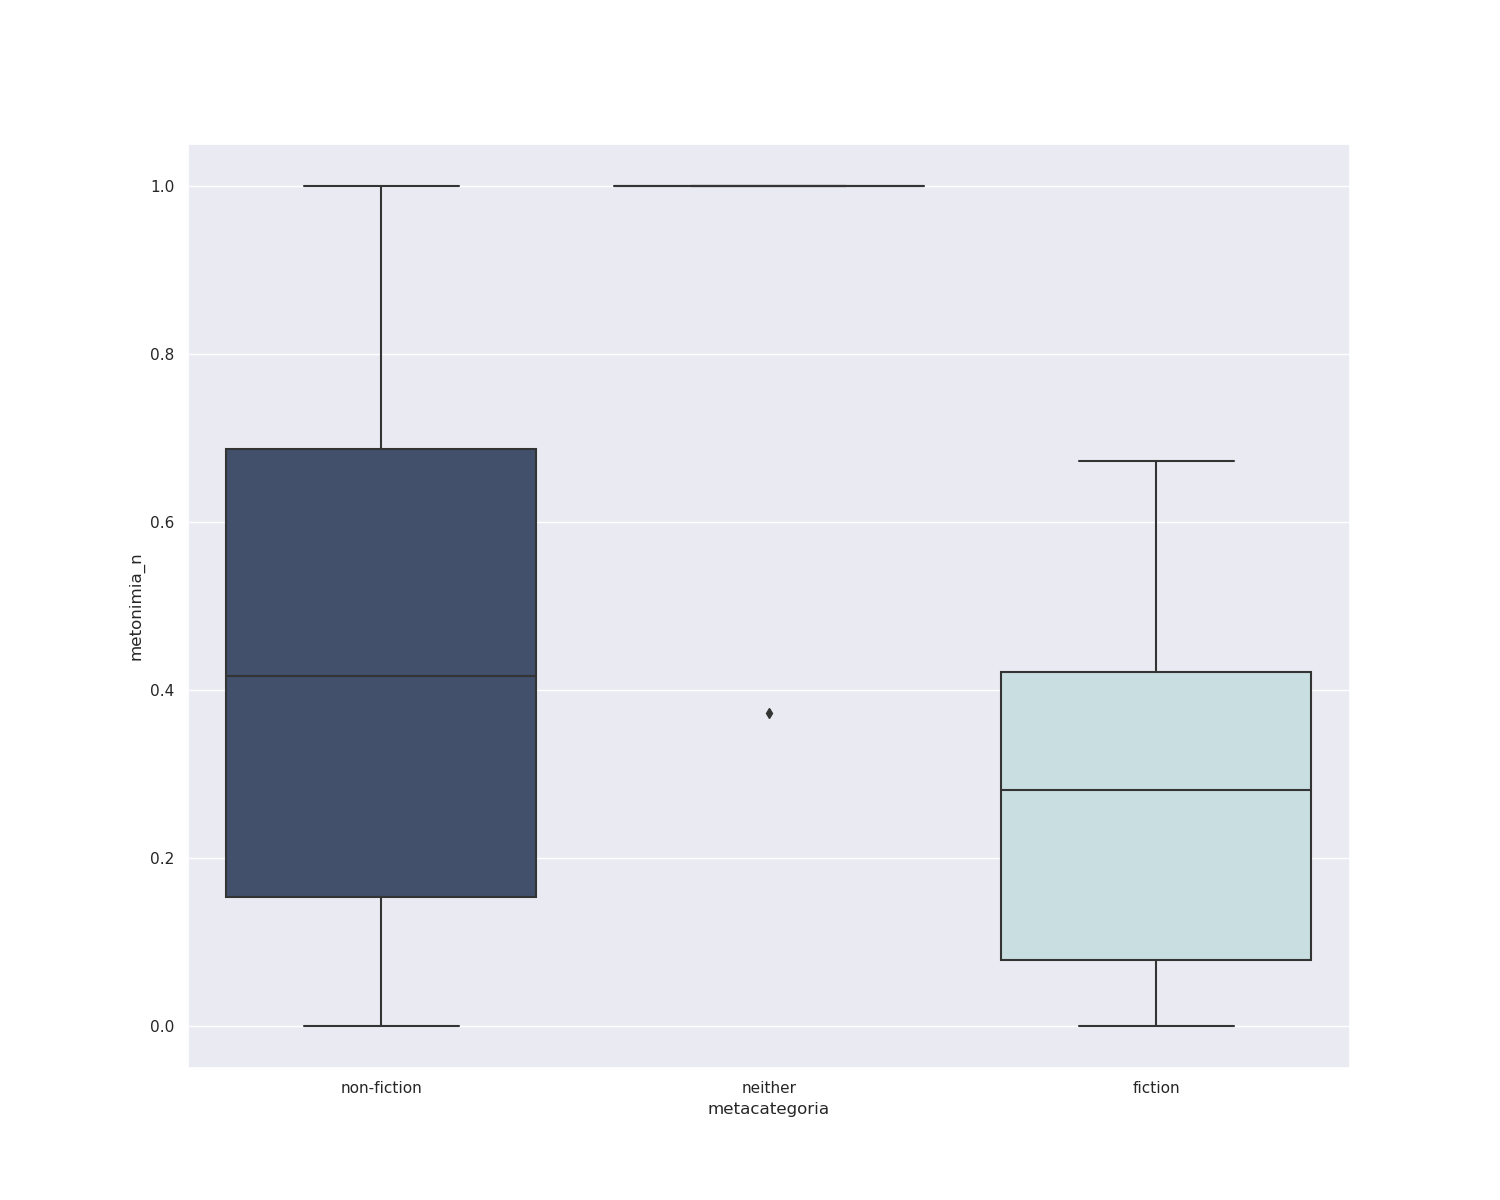
\includegraphics[width=0.9\linewidth]{./resultados/graphs/total/metonimia_total.png}
\caption{\label{fig:metonimia_total} Índice metonímico por metacategoria a través de muestras }
\end{figure}
\end{column}
\end{columns}
\end{frame}

\section{Evaluación}
\label{sec:orgf5b51e0}
\begin{frame}[label={sec:org3baec01}]{Evaluación}
\begin{columns}
\begin{column}{0.48\columnwidth}
  \begin{block}{Criterios cualitativos}
  \begin{table}[H]
  

      \begin{tabular}{|l|l|l}
      \hline
	 Criterio     &  Evaluación \\ \hline
         H_{1}  & Cumplió  \\
         H_{2}  & Cumplió\\
        H_{3}  & No cumplió \\
        H_{4}  & Cumplió\\
\hline
      \end{tabular}

  \end{table}
  \end{block}
\end{column}

\begin{column}{0.48\columnwidth}
\begin{block}{Criterios cuantitativos}
 \begin{table}[H]


     \begin{tabular}{|l|l|l|}
     \hline
	Indicador     &  F & p-value \\ \hline
        Metafora  & 51.41 & 9.81^{-10}  \\
        Metonimia  & 4.32 & 0.04 \\
        \hline

     \end{tabular}

 \end{table}
\end{block}
\end{column}
\end{columns}
\end{frame}

\section{Conclusiones}
\label{sec:org4b62e72}
\begin{frame}[label={sec:org61b44f8}]{Conclusiones}
El modelo propuesto:

\begin{enumerate}
\item produce valores cuantitativos capaces de 'distinguir'
significativamente entre dos metacategorias: los textos de
ficción y los de no-ficción,
\end{enumerate}
\begin{enumerate}
\item parece avalar las observaciones de Jakobson en torno a la relación
de la metonimia con el polo 'Realista' (periódicos, reportes,
artículos, etc) y la metáfora con el polo del 'Romanticismo'
(historias, fábulas, fantasía, etc),

\item tiene algunas ventajas y desventajas con respecto a un enfoque de
Machine Learning. Como ventaja, no se requiere un \emph{training
set}. Como desventaja, el valor de los índices debe ser comparado
entre textos según un contexto dado por el corpus de referencia.
\end{enumerate}
\end{frame}

\begin{frame}[label={sec:orgbf723da}]{Trabajo futuro}
\begin{block}{Mejoramiento del algoritmo}
\begin{itemize}
\item Utilizar Tf-idf para matizar mejor el índice metafórico.
\item Hacer el índice metafórico sensible a los casos donde una palbra se use por debajo del promedio de uso.
\item Hacer el cálculo de similitud del índice metonímico con sílabas o fonemas.
\item Ofrecer la capacidad de personalizar la red semántica.
\end{itemize}
\end{block}

\begin{block}{Mejoramiento de evaluación}
\begin{itemize}
\item Aumentar el número de muestras hasta agotar el Corpus de Brown.
\item Repetir el mismo diseño experimental en el Corpus de LOB, que tiene las mismas categorías que el de Brown.
\item Utilizar los valores de los índices dentro como una característica en un escenario de Machine Learning.
\end{itemize}
\end{block}
\end{frame}

\begin{frame}[label={sec:orgf317906}]{Bibliografía}
\bibliographystyle{ieeetr}
\bibliography{biblio}
\end{frame}
\end{document}